\documentclass[a4paper]{article}

\def\npart{III}

\def\ntitle{Ramsey Theory}
\def\nsheet{I}

\def\ndate{\today}

\input{header}

\let\SO\undefined
\usepackage{tkz-graph}

\newcommand{\shadow}{\partial}
\renewcommand{\P}{\mathbb P}

\begin{document}
	\begin{titlepage}
  \begin{center}
%    \includegraphics[width=0.6\textwidth]{logo.jpg}\par
    \vspace{2cm}
    {\scshape\huge University of \par
      \Huge Cambridge \par}
    \vspace{1cm}
    {\scshape\huge Mathematics Tripos \par}
    \vspace{2cm}
    {\huge Part \npart \par}
    \vspace{0.6cm}
    {\Huge \bfseries \ntitle \par}
    \vspace{0.6cm}
    {\huge Example Sheet \nsheet \par}
    \vspace{1.2cm}
    {\Large\ndate \par}
    \vspace{2cm}
    
    {\large \emph{Solutions by } \par}
    \vspace{0.2cm}
    {\Large \scshape Joshua Snyder}
 \end{center}
\end{titlepage}
	
	\subsection*{Introduction}
	These are written solutions to \ntitle  Example Sheet \nsheet. Solutions are written based on those seen in examples classes and may contain errors from the author.
	\subsection*{Questions}

	% Question 1	
	\begin{question}[Question 1]
	How many combinatorial lines are there in $[m]^n$
	\end{question}
	
	\begin{proof}[1st Solution]
		Each coordinate can take a fixed value in $\{1,..,m\}$ or it can be an active coordinate. Thus for each coordinate there are $m+1$ choices, so there are $(m+1)^n$ active coordinates.
	\end{proof}
	\begin{proof}[2nd Solution]
	Let $f(m,n) = /  \#$ of combinatorial lines, then:
	\[f(m,n) = \sum_{i = \#  \text{active coordinates}} { {n \choose i}1^{i}m^{n-i}} = (m+1)^n\]
	\end{proof}
	\begin{remark}
		As well as being a shorter proof, the first is a better way to think of combinatorial lines in $[m]^n$.
	\end{remark}
	
	% Question 2
	\begin{question}[Question 2]
	Show that $HJ(2,k) = k$ for all $k$
	\end{question}
	\begin{idea}
	Two things to show, $HJ(2,k) \leq k$ and $HJ(2,k) > k-1$. One direction is a proof, the other is a bad colouring.
	\end{idea}
	\begin{proof} $ $\newline
	\begin{description}
	\item \underline{$H(2,k) > k-1 \ (\text{Bad Colouring})$:} Colour $x$ by the number of ones in $\{0,1\}^{k-1}$ then cannot have any combinatorial line since no adjacent $x, y$ are the same colour.
	\item \underline{$HJ(2,k) \leq k \ (\text{Proof})$:} If we can find $k+1$ things, any two of which form a combinatorial line, then we are done. Consider the set
	\[\{(0,0,...,0),(0,0,...,1), (0,0,...,1,1), (0,...,1,1,1), (1,1,...,1)\}\]
Any two of these form a combinatorial line.

	\end{description}
	
	\end{proof}
	
	% Question 3
	\begin{question}[Question 3]
	Let $A$ be an infinite subset of the plane, with no three points collinear. Prove that $A$ contains a set of 2019 points forming a convex 2019-gon.
	\end{question}
	\begin{proof}[Solution 1]
	2-colour $A^{(4)}$ by colouring a 4-set CONVEX if the points form a convex 4-gon. Else colour them NON-CONVEX.\\
	Ramsey's theorem for r-sets implies that there exists an infinite monochromatic subset of $A^{(4)}$. Suppose this is NON-CONVEX, then it must be of the following form:\\
	\begin{figure}[H]
	\centering
	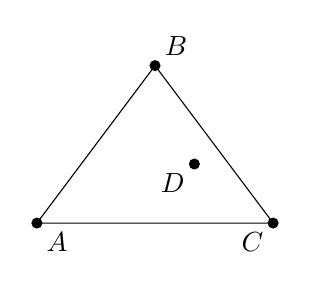
\begin{tikzpicture}
\coordinate [label={below right:$A$}] (A) at (0, 0);
  \coordinate [label={above right:$B$}] (B) at (1.5, 2);
  \coordinate [label={below left:$C$}] (C) at (3, 0);
  \coordinate [label={below left:$D$}] (D) at (2, 0.75);
  
   \foreach \n in {A,B,C,D} \fill [black] (\n)
   circle (2pt) node [below] {};   
  \draw (A) -- (B) -- (C) -- (A);
	\end{tikzpicture}
	\end{figure}
	Adding a 5th point anywhere leads to a convex 4-gon, this can be shown rigorously by splitting the triangle into six regions. Thus there is an infinite CONVEX subset of $A^{(4)}$. Then we are done since we can take any 2019 points and they must form a convex 2019-gon (Suppose not, then there exists a NON-CONVEX 4-gon by triangulating any 2019 points in our set)
	\end{proof}
	\begin{proof}[Solution 2]
	WLOG assume $A$ is countable. Rotate the points in $A$ such that no two lie on the same vertical line. This is possible since there are uncountably many rotations and only countably many points. Now the points in $A$ represent a function and we can colour the 3-sets of $A$ HAPPY if they form a smile and UNHAPPY if they form a frown. Then we are done by Ramsey for 3-sets.
	\end{proof}
	
	\begin{remark}
	If we were using the finite versions of Ramsey for r-sets and wanted to find a smaller bound on the minimum n such that we can make this work, the second proof would give a lower bound since it requires one less induction to prove Ramsey for 3-sets vs Ramsey for 4-sets.
	\end{remark}
	
	% Question 4
	\begin{question}[Question 4]
	Let $c$ be a 2-colouring  of the finite subsets of $\mathbb{N}$. Must there exist an infinite $M \subset \mathbb{N}$ such that, for each $r$, the colouring $c$ is constant on $M^{(r)}$?
	\end{question}
	\begin{idea}
	We want to find a bad colour. Lets ensure one by one that $1 \not\in M$, $2 \not\in M$,...
	\end{idea}
	\begin{proof}
	We ensure that $1 \not\in M$ by letting:
	\[c(i) = \begin{cases} 
      RED & i=1 \\
      BLUE & i\not=1
   \end{cases}
\]
Now we ensure $2 \not\in M$ by letting:
	\[c(ij) = \begin{cases} 
      RED &2 \in \{i,j\} \\
      BLUE & otherwise
   \end{cases}
\]
We continue this by colouring the $r$-sets $X \in \mathbb{N}^{(r)}$:
	\[c(X) = \begin{cases} 
      RED &r \in X \\
      BLUE & otherwise
   \end{cases}
\]
Now suppose there is an infinite monochromatic set $M$ with the desired property, then $M$ cannot be RED else it is just $\{1\}$ which is not infinite, thus $M$ must be BLUE. Then since $r$-set in $M^{(r)}$ contains $r$, $M$ must be empty. Contradiction.
	\end{proof}
	
	% Question 5
	\begin{question}[Question 5]
	Prove that $\{0,1\}^{\mathbb{N}}	$ (with the product topology) is compact.
	\end{question}
	\begin{proof}
	Need to review this, I am unsure of the proof or really what the question is asking.
	\end{proof}
	
	% Question 6
	\begin{question}[Question 6]
	By mirroring the proof of van der Waerden's theorem for arithmetic progressions of length 3, show that whenever $\mathbb{N}^2$ is finitely coloured there exist $a,b,r$ such that the set $\{(a,b), (a+r,b), (a, b+r)\}$ is monochromatic. Deduce by a product argument that whenever $\mathbb{N}^2$ is 2-coloured there exist $a,b,r$ such that the square $\{(a,b), (a+r,b), (a, b+r), (a+r,b+r)\}$ is monochromatic. Give an explicit $n$ such that whenever $[n]^2$ is 2-coloured there exists a monochromatic square.
	\end{question}
	\begin{proof}
	\end{proof}
	
	% Question 7
	\begin{question}[Question 7]
	Show that for every $m$ there is an $n$ with the following property: whenever ${n}^{2}$ is 2-coloured there exists a monochromatic set $M$ of size at least $m$ satisfying $|M| > \min{M}$.
	\end{question}
	\begin{idea}
	Use a compactness argument to get a contradiction.
	\end{idea}
	\begin{proof}
	Suppose not. Then by compactness we get a 2-colouring of the naturals with no $M$ s.t $|M| > \min M$. However by Infinite Ramsey there is an infinite monochromatic set, say $N$. Pick a point in this monochromatic set say $m$, then pick the next $m$ points in $N$ and let these form the set $M$. However then $|M| > \min M$.
	\end{proof}
	
	\begin{remark}
	\begin{itemize}
	\item The exact same argument provides a proof that $\forall m,k,r \ \exists n$ such that when $[m]^{(r)}$ is $k$-coloured there is a monochromatic $M$ with $|M| > \min M$
	\item Compactness arguments like these are a very useful tool.
	\item As an aside, this is an interesting example of a sentence that is true in Peano Arithmetic (PA) but is not provable in PA. This is the Paris-Harrington theorem.
	\end{itemize}
	\end{remark}
	
	% Question 8
	\begin{question}[Question 8]
	Let $A$ be a subset of $\mathbb{N}$ such that, whenever $A$ is finitely coloured, there is a monochromatic arithmetic progression of length $m$. Must $A$ contain an arithmetic progression of length $m+1$?
	\end{question}
	\begin{idea}
	We want a rich enough $A$ such that whenever we $k$ colour $A$ there exists a monochromatic AP of length 3 yet $A$ has no AP of length 4.
	\end{idea}
	\begin{proof}
	Don't understand this proof, need to go through it.
	\end{proof}
	
	% Question 9
	\begin{question}[Question 9]
	Let $\mathbb{N}$ be finitely coloured. Must there exist arbitrarily long monochromatic arithmetic progressions having the same common difference?
	\end{question}
	\begin{idea}
	Seems like too much to ask for. Can we find a really weird colouring that doesn't work for any integer periodic difference?
	\end{idea}
	\begin{proof}
	Colour $\mathbb{N}$ as follows:
		\[c(n) = \begin{cases} 
      RED & \frac{x}{\sqrt{2}} \mod 1 > \frac{1}{2}\\
      BLUE & otherwise
   \end{cases}
\]
Then since $\sqrt{2}$ is irrational there is no periodic nature in the integers, so this colouring suffices. Is there a way to make this more rigorous?
	\end{proof}
	\begin{remark}
	\begin{itemize}
	\item Nothing special about $\sqrt{2}$ here, anything irrational would have done fine e.g $\pi$.
	\item Could have also found other colouring, like ones involving colouring based on the number of ones. For an example of this, see the Thue-Morse sequence (This is a good example of a sequence that ruins a lot of properties and such examples are useful to know).
	\end{itemize}
	\end{remark}
	
	% Question 10
	\begin{question}[Question 10 +]
	Let $A$ be an uncountable set and let $A^{(2)}$ be 2-coloured. Must there exist an uncountable monochromatic set in $A$?}
	\end{question}
	
	% Question 11
	\begin{question}[Question 11 +]
	Let $c$ be a colouring of $\mathbb{N}$ using (possibly) infinitely many colours. Prove that, for every $m$, there is an arithmetic progression of length $m$ on which $c$ is either constant or injective.
	\end{question}
\end{document}